\subsubsection{What software methodology are used in your project?}
\label{methodology}

Software development methodology in software engineering is a framework that is used to pursue the development of information systems in a very deliberate, structured and methodical way. To find out the overall answer of this question, we report the following results:

\begin{itemize}
\item Software development methodologies (Q 6).
\item Requirements gathering (Q 7).
\item Most time consuming software development activities (Q 8).
\end{itemize}


\paragraph{Software development methodologies}
In our study, as per Figure \ref{fig:methodologies}, we have found that the most-widely used model in Bangladesh is Agile with response rate of 64\%. The next widely-used model is scrum with response rate of 46\%. The other methodologies has lower usage rates, namely: pair programming (20\%), Waterfall (12\%) etc. We anticipated that there might be some relation between the software development method and the most time-consuming development activities.  Some methodology may add extra time in development activities. Thus we have calculated the Cramer's V \cite{Cramer1946}. However, we have not found any significant correlation.

\begin{figure}[h]
\centering
  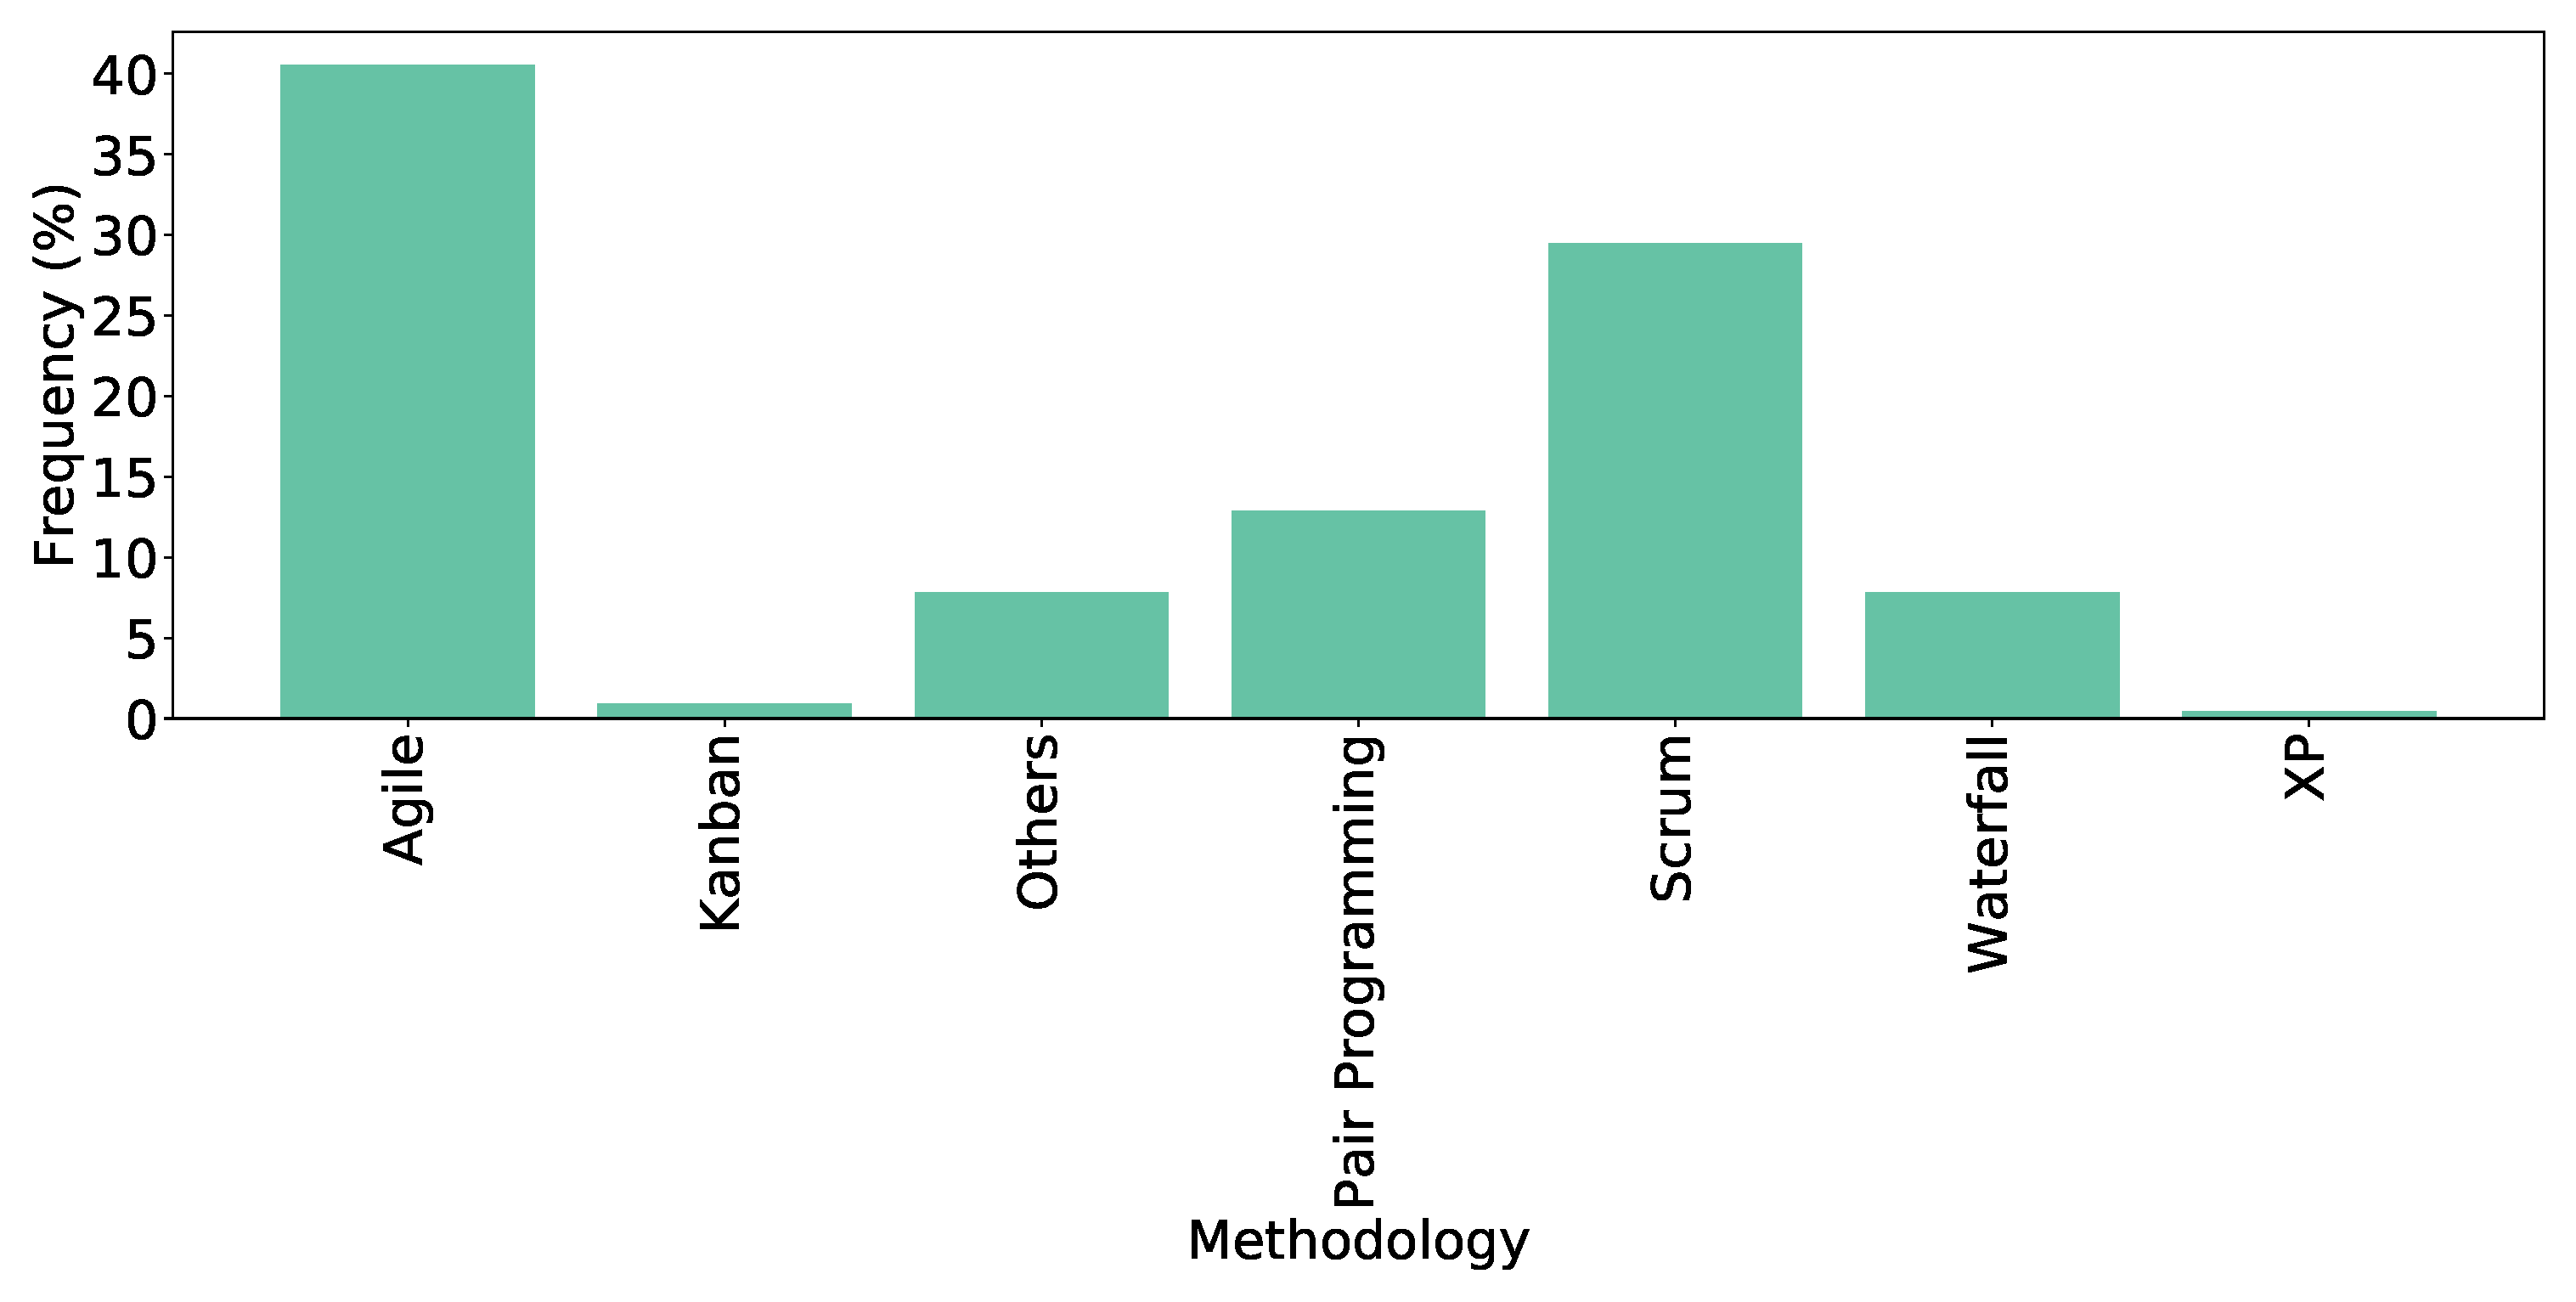
\includegraphics[scale=0.18]{Figures/Respondents_Methodology}
  \caption{Software development methodologies}
  \label{fig:methodologies}
\end{figure}


\paragraph{Requirements Gathering}
The most critical activity that always arises during software development is the collecting requirement of the proposed system. The more clear and details requirements are, the higher the plausibility of building software that conducts the client’s anticipation. Corresponding to Figure \ref{fig:requirements}, using plain text (44\%) and story board (41\%) are the most widely used requirements gathering. The other requirements gathering usage rates are: Use case (36\%), GUI prototype (35\%), grooming session (30\%) etc. This is an important finding that requires further analysis for causes and to analyze the potential effects of not documenting requirements.

\begin{figure}[h]
\centering
  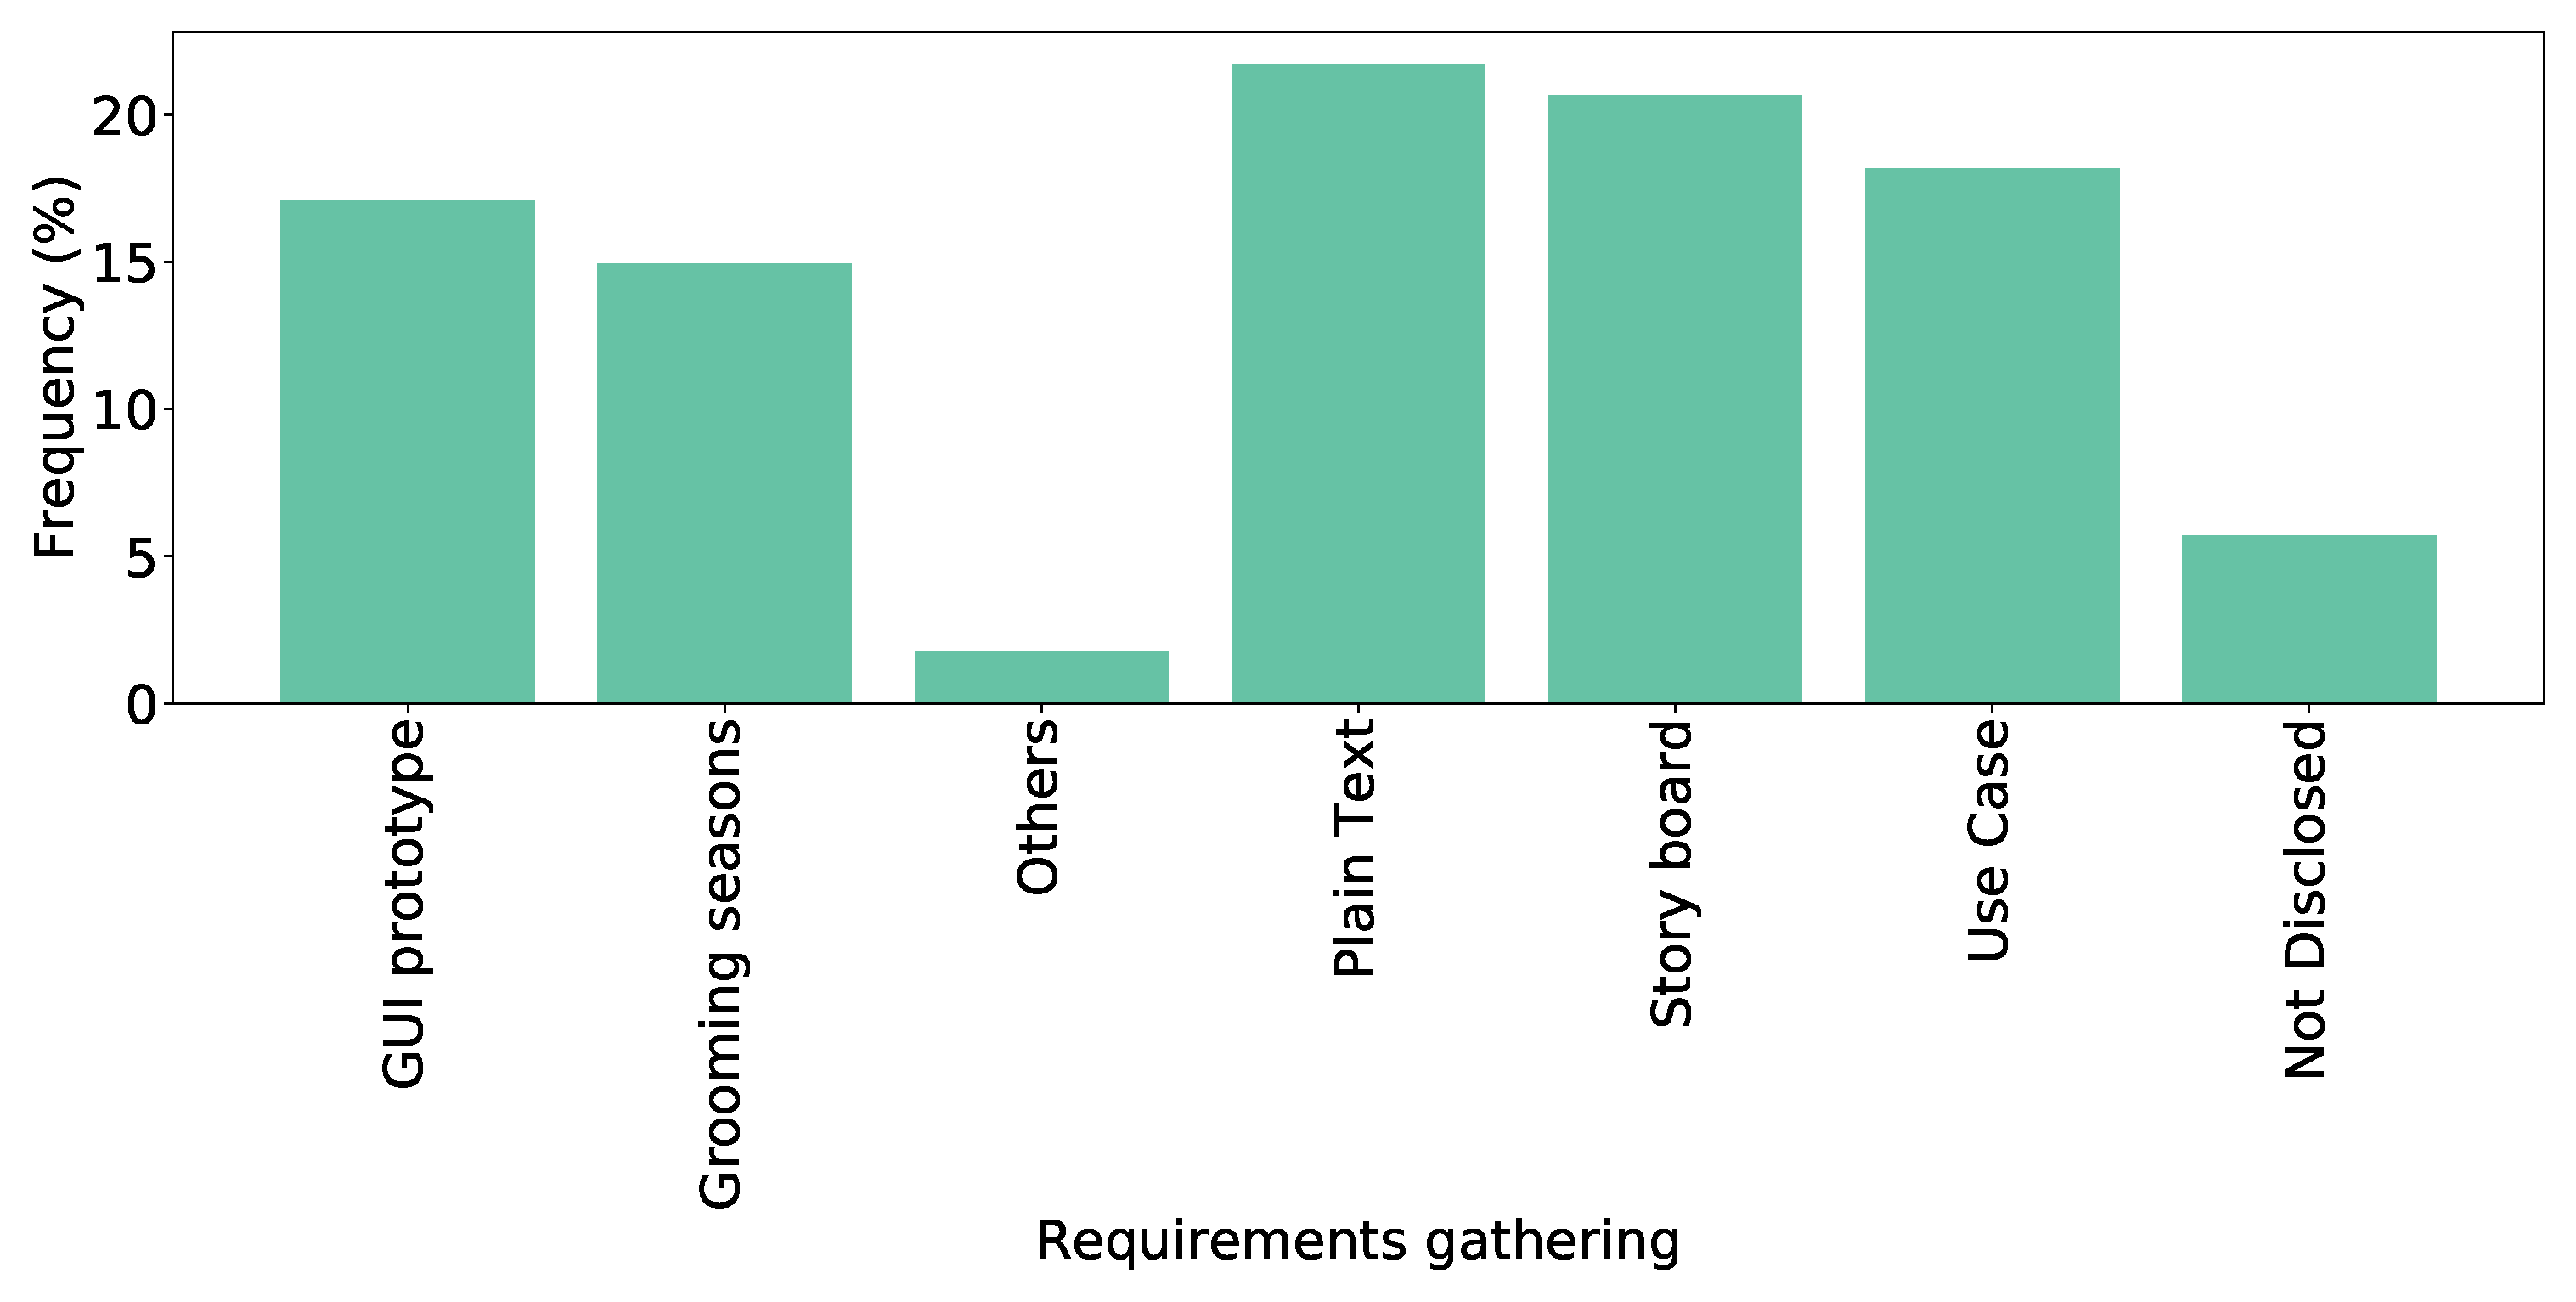
\includegraphics[scale=0.18]{Figures/Requirements_Gathering}
  \caption{Requirements gathering}
  \label{fig:requirements}
\end{figure}


\paragraph{Development activities timeline}
In this section participants were asked about the most time consuming software developing activities they had spend. We have presented their activities based on the percentage of the participants in Figure \ref{fig:activities}. From the Figure \ref{fig:activities}, we see that most of the time spent in implementation stage according to 65\% our respondents and requirement analysis stage requires second most according to 45\% response. The other usages are: Program design (37\%), project planning (30\%), testing (19\%), maintenance (17\%) etc.

\begin{figure}[h]
\centering
  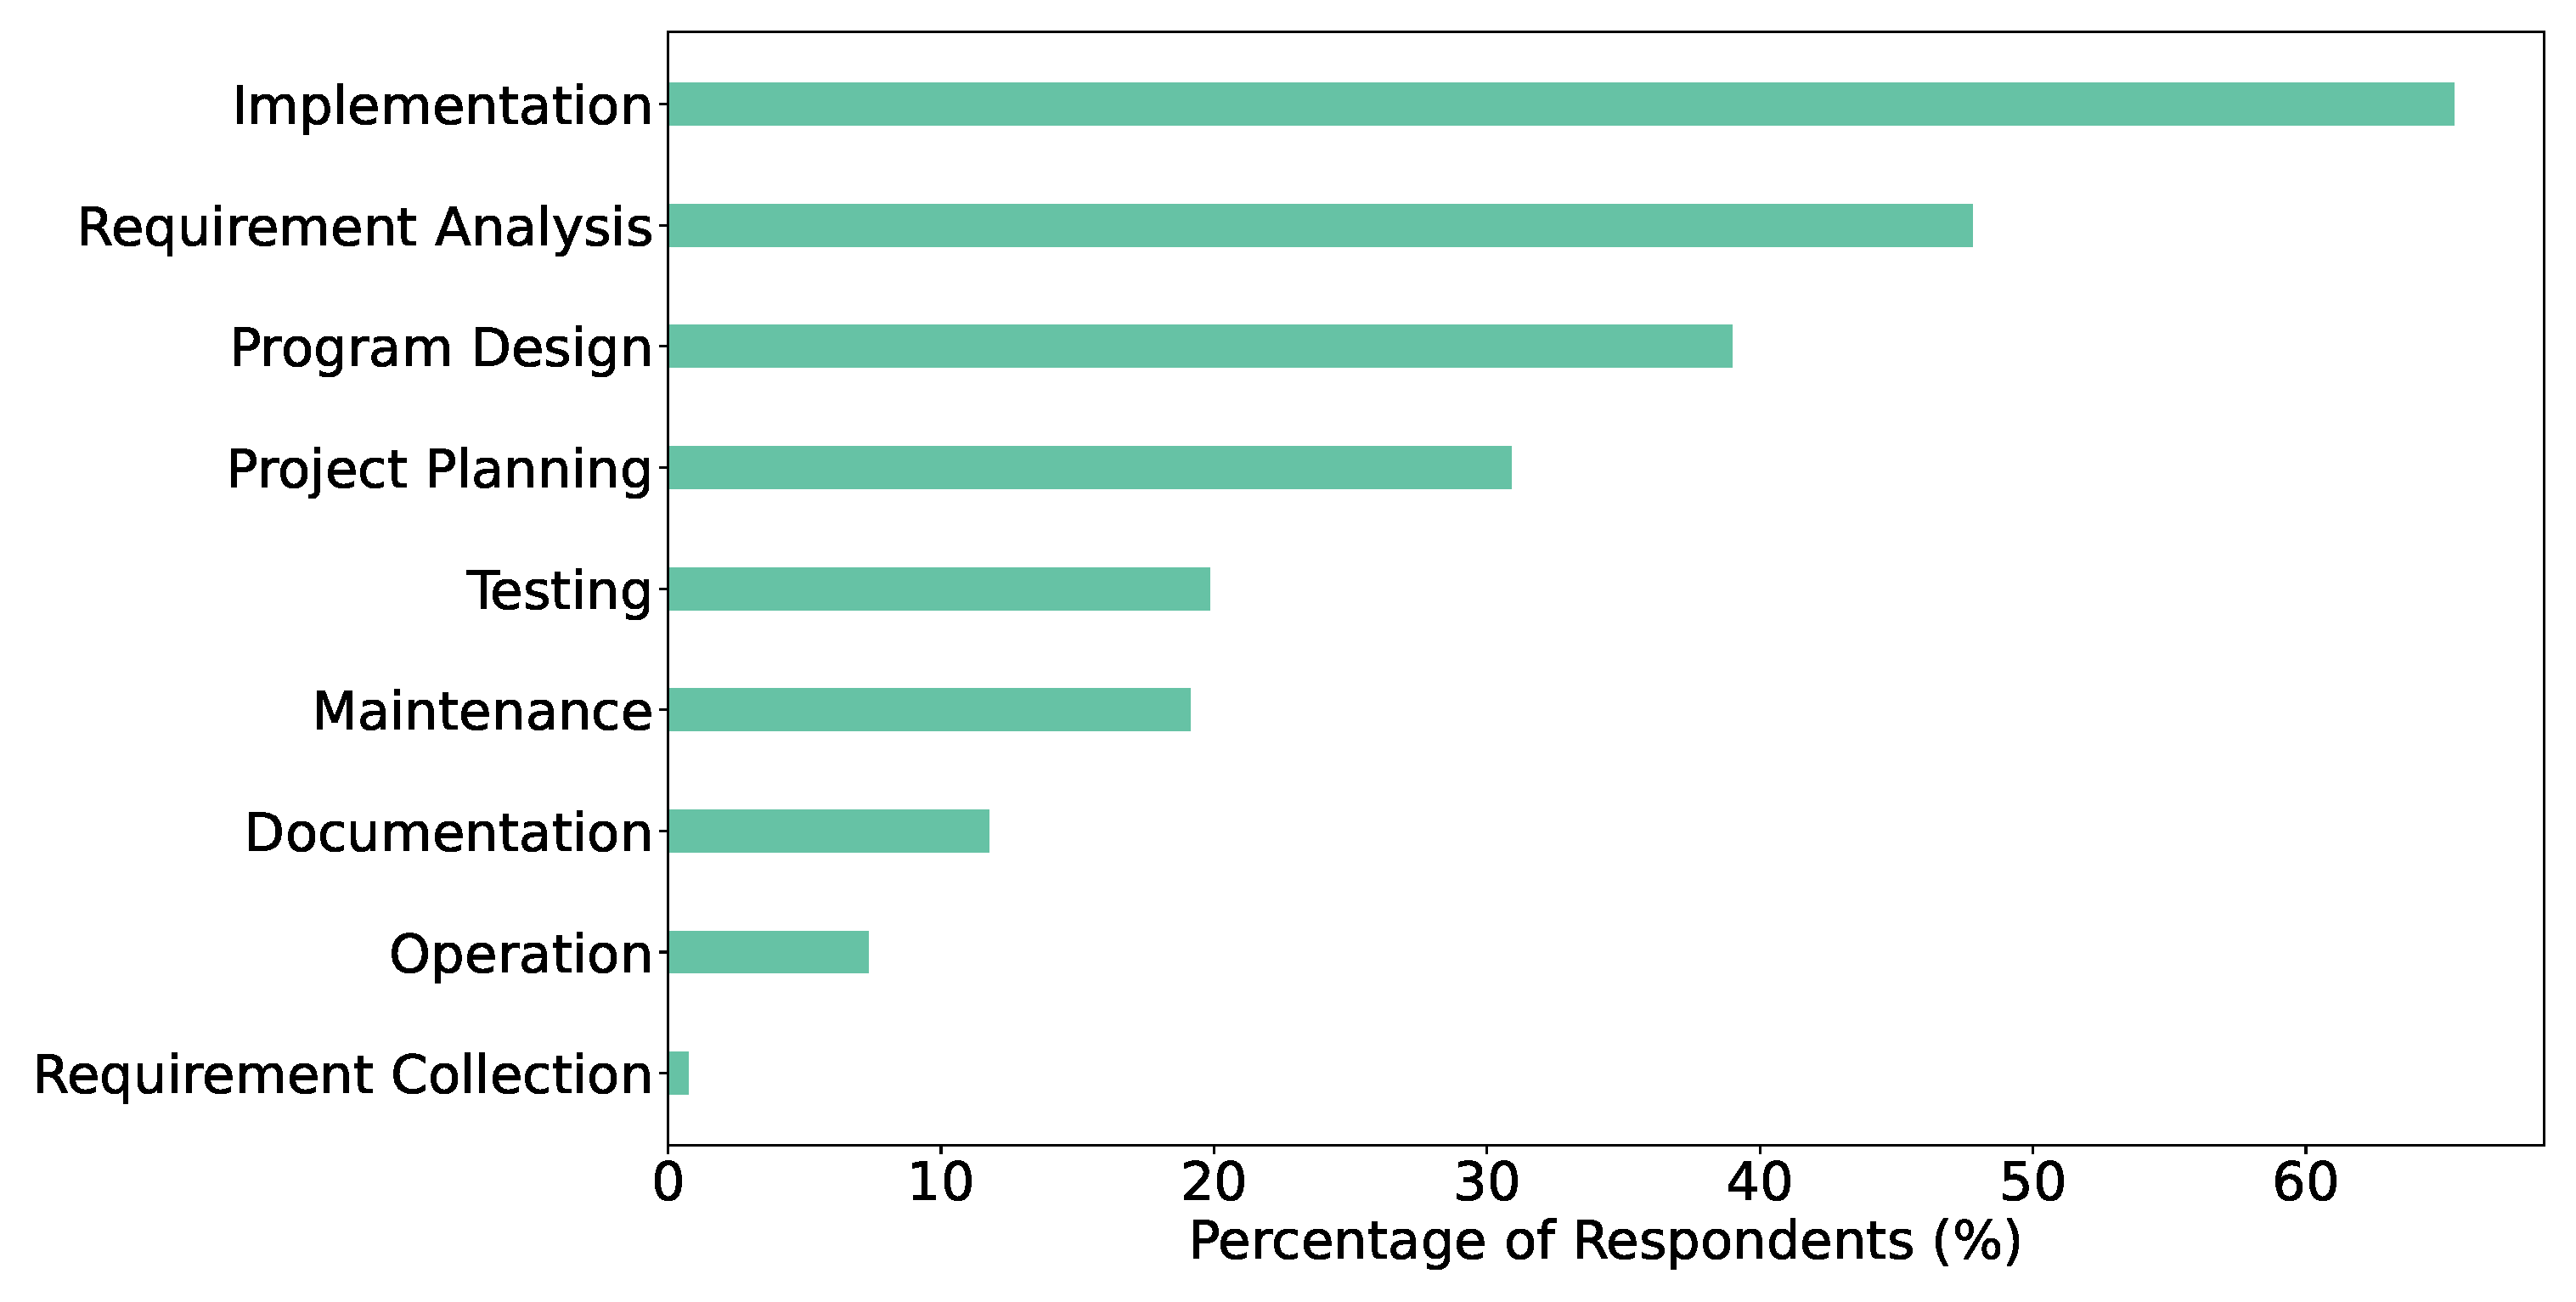
\includegraphics[scale=0.2]{Figures/Respondents_Activities}
  \caption{Software development activities}
  \label{fig:activities}
\end{figure}

We guessed that there might be a relation between developers' experience activity. It is a general idea that senior developers spend most of their time in requirement specification and design activities where junior developers spend their time implementing the solution. We divided our respondents into two groups based on their professional experience. Developers with more than 5 years of experience are considered senior, and others are considered junior developers. The Most spent activity with Developers experience is plotted in Figure \ref{fig:activity and seniority}. We can see that our anticipation is right. Junior developers are mostly engaged in the implementation where senior developers are engaged with requirement specifications.

\begin{figure}[h]
\centering
  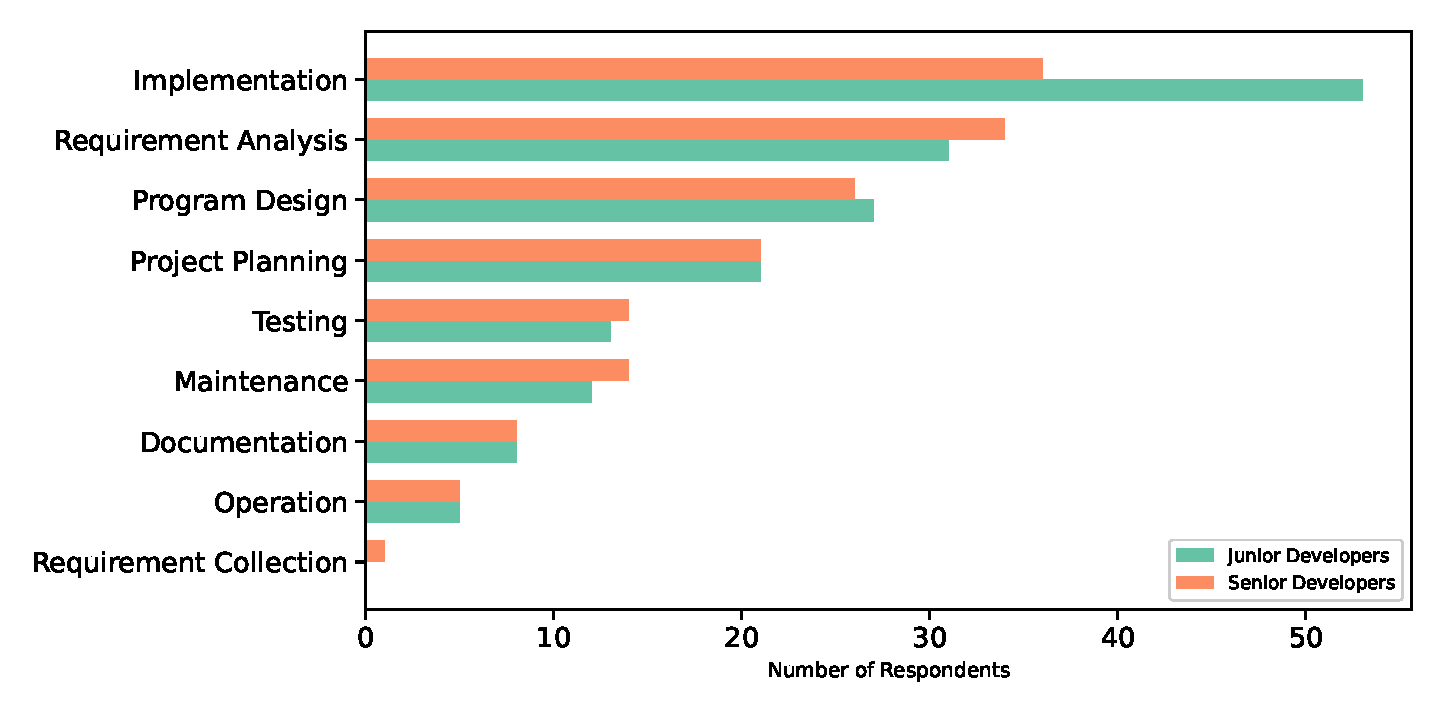
\includegraphics[scale=0.4]{Figures/Activity_and_Seniority.eps}
  \caption{Relation between seniority and activity}
  \label{fig:activity and seniority}
\end{figure}
\partha{In the survey the activity was a multiple choice field. Not sure we can perform any stat. analysis. Will it be theoretically correct?}

\boxtext{Developers of Bangladeshi SE industry generally spend most time on implementation-related activities compared to planning and testing.}
